
\documentclass[
  aspectratio=1610, 
  xcolor={dvipsnames},
  % handout
]{beamer}

\usetheme{metropolis}

\setbeamercolor{background canvas}{bg = white}

\input{macro}

\title{CDCL and Proof Production for (UN)SAT}
\author{Sankalp Gambhir}

\begin{document}

\maketitle

\begin{frame}
  \frametitle{The Problem}

  We have a language, of a countable set of atoms $A = \{x, y, z, \ldots\}$, and
  ways to combine them $x \land y$, $x \lor y$, and $\neg x$ with the usual
  interpretations. These terms form a Boolean algebra.

  \pause
  A \emph{literal} is an atom $x$ or its negation $\neg x$. 
  
  \pause
  A \emph{clause} is a disjunction of literals $C = \neg x \lor y \lor \neg z \lor \ldots$.

  \pause
  A \emph{formula in conjunctive normal form (CNF)} is a conjunction of clauses $F =
  C_1 \land C_2 \land \ldots$.

  % in essence, the formula says, one of these must hold, one of these, and so on.

\end{frame}

\begin{frame}
  \frametitle{The Problem}

  The \emph{(Clausal) Boolean Satisfiability Problem (Clausal SAT)} is the
  problem of determining whether a given formula $F$ in CNF is satisfiable,
  i.e., whether there exists a mapping \(\sigma: A \to \{0, 1\}\) (or
  \(\mathbb{B}\)) such that \(F\sigma = 1\) under the usual interpretation of
  the two-element Boolean algebra.

  Typically, we are also interested in producing such a mapping, if it exists.

\end{frame}

\begin{frame}[fragile]
  \frametitle{Recap}

  We looked at interpreting the SAT problem very plainly as a reading of the
  definition:

  \begin{lstlisting}
    def checkSat(f: Formula[Prop]): SatResult[Prop] =
      f.frees.toSet.subsets
        .find(f.evaluateUnder) match
        case Some(s) => Sat(s)
        case None => Unsat
  \end{lstlisting}

\end{frame}

\begin{frame}[fragile]
  \frametitle{Recap}

  We tried to come up with a way to frame this as a decision procedure that
  checks variables one by one, wherein we got a branching procedure:
  
  \begin{lstlisting}[basicstyle=\ttfamily\scriptsize]
    def checkSat(f: CNF[Prop]): SatResult[Prop] =
      def rec(clauses: Set[Clause[Prop]], choices: List[Literal[Prop]], frees: List[Prop]): SatResult[Prop] =
        if clauses.isEmpty then Sat(choices)
        else if clauses.exists(_.isEmpty) then Unsat
        else if frees.isEmpty then Unsat
        else
          // decide
          val x = frees.head
          val rest = frees.tail
          // branch
          lazy val pos = 
            rec(clauses.substitute(x, true), Pos(x) :: choices, rest)
          lazy val neg = 
            rec(clauses.substitute(x, false), Neg(x) :: choices, rest)
          pos.orElse(neg)
      rec(f.clauses, Nil, f.frees)
  \end{lstlisting}

\end{frame}

\begin{frame}
  \frametitle{What is our search space?}

  % bdd as the search space

  % prev algorithm is DFS

  % however, looking at this, we can see that we didn't always have to go all
  % the way to the root to know we have failed (or succeeded), since all leaves
  % in this and this segment are the same. So as Shardul suggested before, we
  % can reduce our formula at each step to figure out if we are done early.
  
  % this is typically done by unit propagation (which is part of the reason
  % clausal forms are preferred)

  % we will see precisely how to make good use of this partial information a bit
  % later

\end{frame}

\begin{frame}
  \frametitle{Proof Production}

  Extension of the original problem: with an answer to the SAT problem, can you
  also supply a \emph{certificate} for the answer that can be efficiently
  checked?

  \pause
  \textbf{On SAT:} \pause
  The model is a certificate. We can substitute the model into the formula
  and check in linear time whether the formula indeed evaluates to true.

  \pause
  \textbf{On UNSAT:} \pause
  % what have we shown, exactly? What is our 'no' worth?
  %
  % concretely, reading the problem definition, we have shown that there is no
  % mapping that satisfies the formula. How do you convince someone else of
  % this?
  %
  Note that if \(f_1 \iff f_2\), then \(\forall \sigma: A \to \mathbb{B}.\;
  f_1\sigma = f_2\sigma\). 

  If \(\not\exists \sigma. f\sigma = 1\), then \(f \iff \bot\). Since \(\bot
  \Rightarrow f\) always holds, our 'no' is actually stating that \(f
  \Rightarrow \bot\).

  A certificate for this is a proof of \(f \Rightarrow \bot\), or a
  \emph{refutation}.

\end{frame}
\begin{frame}[fragile]
  \frametitle{Where do proofs squeeze in?}
  
  \begin{lstlisting}[basicstyle=\ttfamily\scriptsize]
    def checkSat(f: CNF[Prop]): SatResult[Prop] =
      def rec(clauses: Set[Clause[Prop]], choices: List[Literal[Prop]], frees: List[Prop]): SatResult[Prop] =
        if clauses.isEmpty then Sat(choices)
        else if clauses.exists(_.isEmpty) then Unsat
        else if frees.isEmpty then Unsat
        else
          // decide
          val x = frees.head
          val rest = frees.tail
          // branch
          lazy val pos = 
            rec(clauses.substitute(x, true), Pos(x) :: choices, rest)
          lazy val neg = 
            rec(clauses.substitute(x, false), Neg(x) :: choices, rest)
          pos.orElse(neg)
      rec(f.clauses, Nil, f.frees)
  \end{lstlisting}

\end{frame}

\begin{frame}
  \frametitle{Using Partial Information}

  \begin{multicols}{2}

  \begin{align*}
    c_1 && \neg p_4 \lor p_5 \\
    c_2 &&  \neg p_4 \lor p_3 \lor p_7 \\
    c_3 && \neg p_5 \lor p_6 \\
    c_4 && \neg p_3 \lor \neg p_6 \\
    c_5 && p_4 \lor p_7 \lor \neg p_5 \\
    c_6 && p_5 \lor p_3 \\
    c_7 && p_5 \lor \neg p_3 \lor \neg p_2 \\
    c_8 && \neg p_1 \lor \neg p_2 
  \end{align*}

  \columnbreak

  \pause
  \begin{center}
    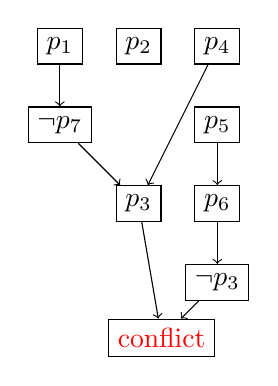
\begin{tikzpicture}
      \node[draw, rectangle] (p1) {\(p_1\)};
      \node[draw, rectangle, below of = p1] (np7) {\(\neg p_7\)};

      \node[draw, rectangle, right of = p1] (p2) {\(p_2\)};

      \node[draw, rectangle, right of = p2] (p4) {\(p_4\)};
      \node[draw, rectangle, below of = p4] (p5) {\(p_5\)};
      \node[draw, rectangle, below of = p5] (p6) {\(p_6\)};

      \node[draw, rectangle, left of = p6] (p3) {\(p_3\)};
      \node[draw, rectangle, below of = p6] (np3) {\(\neg p_3\)};

      \node[draw, rectangle, below left of = np3] (cfl) {\textcolor{red}{conflict}};

      \draw[->] (p1) -- (np7);
      \draw[->] (p4) -- (p3);
      \draw[->] (np7) -- (p3);
      \draw[->] (p5) -- (p6);
      \draw[->] (p6) -- (np3);
      \draw[->] (p3) -- (cfl);
      \draw[->] (np3) -- (cfl);
    \end{tikzpicture}
  \end{center}

  \pause
  We can say more concretely, \(\neg p_1 \lor \neg p_4\), and jump back.
  % but jump back where?
  %
  % let's jump back. if we go back one decision, we are stuck again, and we are forced to jump back once more etc.
  % 
  % so, we j7ump back to the second last decision that caused this conflict.
  % note that because we know this new clause, we immediately choose a new value for p4 and move on. 
  \end{multicols}
\end{frame}

\begin{frame}
  \frametitle{CDCL}

  \pause
  That was CDCL, thanks and bye.

  \pause
  \begin{center}
    Conflict-driven clause learning
  \end{center}

  % why is it considered a different algorithm with its own name and nto an
  % optimization?

  % well, the best arugment I've found is that CDCL produces massively different
  % access patterns and explores the search space much mroe dynamically, which
  % author of said text characterized as the fingerprint of an algorithm.

\end{frame}

\begin{frame}
  \frametitle{Proof production for CDCL}

  Question 1: what is a conflict? What are we saying, precisely, when we
  discover a conflict?

  \pause
  Question 2: what about the little inferences we made at each step?

  \pause
  Question 3: how do we compose these together?

  \pause
  Question 4: how do we stop? (or even, do we?)

\end{frame}

% \begin{frame}
%   \frametitle{Conflicts}

%   When we found the conflict before, what we really said was:

%   \begin{gather*}
%     \AxiomC{}
%     \RightLabel{Assumption}
%     \UnaryInfC{\(p_1 \vdash p_1\)}
%     \AxiomC{}
%     \RightLabel{Assumption}
%     \UnaryInfC{\(p_4 \vdash p_4\)}
%     \AxiomC{\(\Phi\)}
%     \TernaryInfC{\(\bot\)}
%     \Displayproof
%   \end{gather*}

% \end{frame}

\begin{frame}

  \begin{center}
    \Huge Thank you!
  \end{center}

\end{frame}

% we will hopefully understand and come back to conjugate hylomorphisms at some
% point

% open questions and motivations
%% we kinda know while loops can emulate more or less what goto did, in practice
%% what is the analogue for recursion? 
%% there are clearly non catamorphic functions
%% what about non cata/ana/hylomorphisms?
%% can we represent partial functions (sometimes non terminating)? should we?

%% questions for my research
%% what kind of recursive schemes can we efficiently verify?
%% we know that Horn clauses over datatypes + catamorphisms are doable (kinda)
%% other classifications (sufficiently surjective (Suter / Dotta / Kuncak))

\end{document}
